\documentclass{VUMIFPSkursinis}
\usepackage{algorithmicx}
\usepackage{algorithm}
\usepackage{algpseudocode}
\usepackage{amsfonts}
\usepackage{amsmath}
\usepackage{bm}
\usepackage{caption}
\usepackage{color}
\usepackage{float}
\usepackage{graphicx}
\usepackage{listings}
\usepackage{float}
\usepackage{subfig}
\usepackage{wrapfig}
\usepackage[hidelinks]{hyperref}
\usepackage{todonotes}

% Titulinio aprašas
\university{Vilniaus universitetas}
\faculty{Matematikos ir informatikos fakultetas}
\department{Programų sistemų katedra}
\papertype{Programų kūrimo proceso laboratorinis darbas}
\title{Įmonės ,,Mėnuliukų technologijos" programų kūrimo proceso brandos vertinimas}
\titleineng{Maturity assessment of the development process of the ,,Moon Technologies" company}
\status{4 kurso 3 grupės studentai}
\author{Matas Savickis, Justas Tvarijonas, Džiugas Mažulis}
\secondauthor{Greta Pyrantaitė, Andrius Bentkus}

\supervisor{Saulius Ragaišis, Doc., Dr.}
\date{Vilnius – \the\year}

% Nustatymai
% \setmainfont{Palemonas}   % Pakeisti teksto šriftą į Palemonas (turi būti įdiegtas sistemoje)
\bibliography{bibliografija}

\begin{document}
\maketitle

\tableofcontents

\sectionnonum{Įvadas}
	Šiame dokumente aprašysime dabartinio ,,Mėnuliukų technologijos" įmonės programų kūrimo proceso pagerinimą. 
	Dabar nei vienas iš aprašytų procesų nepasiekia pirmo lygio.
	Šiuo darbu sieksime, kad po proceso pagerinimo trys procesai pasiektų pirmą PKP brando lygį.
	\begin{figure}[htbp]
		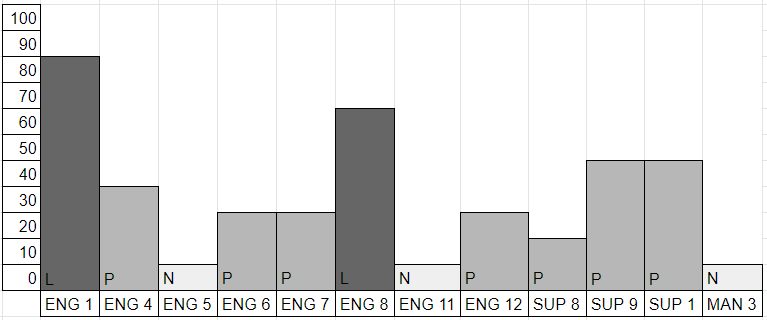
\includegraphics[scale=1]{img/ProcPries}
		\caption{PKP brandra prieš pagerinimą} % Antraštė įterpiama po paveikslėlio
		\label{img:pkpPries}
	\end{figure}

\section{Reikalavimų išsiaiškinimo (ENG 1) proceso pagerinimas}
\section{Programinės įrangos testavimo (ENG 8) proceso pagerinimas}	
\section{Kokybės užtikrinimo (SUP 1) proceso pagerinimas}


\end{document}
